%%%%%%%%%%%%%%%%%%%%%%% Grundeinstellungen %%%%%%%%%%%%%%%%%%%%%%%%%%%
% 'Artikel' Dokumentenklasse und Standardschriftgröße  
\documentclass[11pt,landscape]{beamer}


% Setzt das Papierformat und den Rand auf 2.5cm                                                      
%\usepackage[paper=a4paper,left=2.5cm,right=2.5cm,top=2.5cm,bottom=2.5cm]{geometry}  

% Setzt die Einrückung von Absätzen auf gegebenen Abstand
\setlength{\parindent}{0mm}

% Legt Zeilenabstand fest                                                         
%\usepackage[onehalfspacing]{setspace}                                               

% Legt FontKodierung fest
\usepackage[T1]{fontenc}

% Legt Zeichenkodierung fest                                                            
\usepackage[utf8]{inputenc}                                                         

% Neue Deutsche Rechtschreibung
\usepackage[ngerman]{babel}  

% Versieht Referenzen mit Bezeichnung des Objektes                                                      
%\usepackage[ngerman]{varioref}   

% Empfohlener T1-Font für deutsche Texte                                               
\usepackage{lmodern} 

% Deutsche Zitate mit \enqoute{},\enqoute*{} 
\usepackage[babel,german=quotes]{csquotes}

%Einstellungen für Bibliographien mit "biber"                                                              
\usepackage[backend=biber,sorting=none]{biblatex}

%%%%%%%%%%%%%%%%%%%% Seitenlayout %%%%%%%%%%%%%%%%%%%%%%%%%%%%%%%%%%%%

% Ermöglicht detailierte Bearbeitung der Kopf- und Fußzeile
\usepackage{fancyhdr} 

% Setzt Kopf und Fußzeile zurück                                                              
%\fancyhf{} 	     
         
% Höhe der Kopfzeile                                                          
%\setlength{\headheight}{28.0pt}   

% Höhe der Fußzeile                                                  
%\setlength{\footskip}{18.0pt}                                                      

% Dicke des Kopfzeilentrennstrichs
%\renewcommand{\headrulewidth}{.5 pt}     

% Dicke des Fußzeilentrennstrichs                                     
%\renewcommand{\footrulewidth}{.5 pt}                                                 

%Test ob Variable gesetzt ist oder nicht
%\ifdefined\ExperimentTitle% 
	% Angabe Links-Oben
%	\lhead{\textbf{\ExperimentTitle}}
%\else%
%    \lhead{\textbf{\textcolor{red}{VERSUCHNAME!!!}}}
%\fi%      
                                                            
% Angabe Mitte-Oben
%\chead{}  

% Angabe Rechts-Oben                                                                         
%\rhead{\today}  

% Angabe Links-Unten                                                                    
%\lfoot{}        

% Angabe Mitte-Unten                                                                   
%\cfoot{\textbf{\thepage\ von \pageref{LastPage}}}  

% Angabe Rechts-Unten                                 
%\rfoot{}                                           

% Anwenden des erweiterten Seitenlayouts
%\pagestyle{fancy}      
%%%%%%%%%%%%%%%%%%%%%%% Referenzen %%%%%%%%%%%%%%%%%%%%%%%%%%%%%%%%%%%

% Macht die letzte Seitenzahl referenzierbar mit \pageref{Lastpage}
\usepackage{lastpage}

% Ermöglicht Referenzen im Dokument                                                               
\usepackage{hyperref}
	%Keine Hervorhebung der Referenzen
	\hypersetup{hidelinks}

%Verbesserte Referenzen
\usepackage[german]{cleveref}
                                                              
%%%%%%%%%%%%%%%%%%%%%%%% MINT %%%%%%%%%%%%%%%%%%%%%%%%%%%%%%%%%%%%%%%%
% Fügt mathematische Symbole hinzu, setzt Grenzen, Limiten und Indizes unter das Symbol und nicht dahinter
%\usepackage[sumlimits,intlimits,namelimits]{amsmath}  
\usepackage{amsmath}  
% Fügt Symbole wie z.B. Zahlenmengen wie $\mathbb{R}$ hinzu                             
\usepackage{amssymb}    
                                                             
% Beweißumgebung
\usepackage{amsthm}  

% Font für Mathematikumgebung                                                              
\usepackage{amsfonts}    
                                                          
% Verbesserte Gleichungsumgebung mit \begin{empheq}[<Aussehen>]{<Umgebungstyp>} ... \end{empheq}
\usepackage{empheq}      

% Ergänzungen für physikalische Arbeiten
\usepackage{physics}

% Chemische Struktur und Summenformeln mit \ce{<Summenformel>}                                                          
%\usepackage[version=3]{mhchem}  

% Chemische Valenzstrichformeln für ganze Moleküle mit\chemfig{<Molekül-Aufbau>}                                                   
%\usepackage{chemfig}                                                               

% Verbesserte Formatierung von größen mit Einheiten 
\usepackage[binary-units=true]{siunitx}                                                               
	% 'Mal'-Zeichen auf \cdot und Dezimaltrennzeichen auf ',' 
	\sisetup{locale = DE,prefixes-as-symbols = true}                                   
                                                                            
	% Vereinfachtes eintragen von Unsicherheiten mit '42.6(4)' --> '42.6 +/- 0.4'          
	\sisetup{separate-uncertainty = true}                                                                                                                    

 
                                                            
% Fügt verbesserte Vektorpfeile hinzu \vv{<Vektorname>} 
\usepackage[b]{esvect}  

% Brüche mit "/" im Text mit \sfrac{}                                                            
\usepackage{xfrac}

% Darstellung von 2D Feldern 
\usepackage{array}

% Differentialoperatoren,-quotienten und Klammern mit \od[]{}{}, \pd[]{}{}, \del{}, \sbr{}, \cbr{}
\usepackage{commath}

% Pseudocode-Umgebungen 																
\usepackage{algorithmicx}
\usepackage{algpseudocode}

% Einbinden von SourceCode Dateien (listing)
\usepackage{listings}
	% Auswählen der Programmiersprache
	\lstset{language=Python}

%%%%%%%%%%%%%%%%% Seiten- und Floateinstellungen %%%%%%%%%%%%%%%%%%%%%
% Einbinden von Grafiken mit '\includeudegraphics[<Optionen>]{<Grafikpfad>}' und Veränderungen im Text, wie z.B. Schriftfarbe 
\usepackage{graphicx}
\usepackage{xcolor} 
\xdefinecolor{tugreen}{RGB}{128, 186, 38}

% Fügt Möglichkeit für textumflossende Grafiken und Tabellen hinzu \begin{floating<figure/table>}[option]{width} ... \caption ... \end{floatingfigure}                                                              
\usepackage{floatflt}        
\usepackage{wrapfig}

% Ermöglicht das Hinzufügen von Unterabbildung zu einer Abbildung                                                 
%\usepackage{subfig} 

% Verhindert das Wandern von "floating" Umgebungen über eine Bestimmte Grenze (hier: Sections) oder mit \FloatBarrier                                                             
\usepackage[section]{placeins}

% Ermöglicht Zeichnungen im Dokument \begin{tikzpicture} ... \end{tikzpicture}
\usepackage{tikz}  
	% Fügt zusätzlichen Pfeilspitzen hinzu                                                                 
	\usetikzlibrary{arrows}                                                         
	\usetikzlibrary{calc}    
% Besseres Tabellenlayout                                                        
\usepackage{booktabs}

% Skalierbare Umgebung für Tabellen und Bilder
\usepackage[export]{adjustbox}

% Bearbeiten von Bild-/Tabellenunterschriften
\usepackage[font=small,labelfont=bf]{caption}

% Seiten im Querformat mit \begin{landscape}...\end{landscape} 
\usepackage{pdflscape}

% Ermöglicht detailierte Einstellungen an Aufzählungssymbolen
%\usepackage{enumitem} 

% Ermöglicht das Einfügen mehrerer Einträge in eine Tabellenzelle, getrennt von einem '\'
% \backslashbox{<Eintrag unten-links>}{<Eintrag oben-rechts>} TIPP: Leerzeichen                                                          
%\usepackage{slashbox}   

%Einbinden von Textdateien
\usepackage{fancyvrb}
% redefine \VerbatimInput
\RecustomVerbatimCommand{\VerbatimInput}{VerbatimInput}%
{fontsize=\footnotesize,
	%
	frame=lines,  % top and bottom rule only
	framesep=1em, % separation between frame and text
	rulecolor=\color{gray},
	%
	label=\fbox{\color{black} Kenngrößen},
	labelposition=topline,
	%
	commandchars=\|\{\}, % escape character and argument delimiters for
	% commands within the verbatim
	commentchar=\#       % comment character
	}
	
%%%%%%%%%%%%%%%%%%%%%%%%%%%%%%%%%%%%%%%%%%%%%%%%%%%%%%%%%%%%%%%%%%%%%%

% Fügt verbesserte Unterschtreichungen hinzu, z.B. doppelt, gezackt, gewellt, etc. mit \uline{},\uuline{},
\usepackage[normalem]{ulem}                                                                                                               

%Verbesserte Verwendung von Daten
\usepackage{scrdate}

% Zusaätzliche Symbole
\usepackage{pifont}

% Fügt extra Symbole hinzu 
\usepackage{textcomp}  

% Emojis
%\usepackage{styles/coloremoji}
%\Smiley,\Sadey,\Neutrey
\usepackage{tikzsymbols}
\newcommand{\ketsmiley}{\ensuremath{\ket{\Smiley}}}
\newcommand{\brasmiley}{\ensuremath{\bra{\Smiley}}}
\newcommand{\ketneutrey}{\ensuremath{\ket{\Neutrey}}}
\newcommand{\braneutrey}{\ensuremath{\bra{\Neutrey}}}
\newcommand{\ketfrowny}{\ensuremath{\ket{\Sadey}}}
\newcommand{\brafrowny}{\ensuremath{\bra{\Sadey}}}
\newcommand{\ketup}{\ensuremath{\ket{\uparrow}}}
\newcommand{\braup}{\ensuremath{\bra{\uparrow}}}
\newcommand{\ketdown}{\ensuremath{\ket{\downarrow}}}
\newcommand{\bradown}{\ensuremath{\bra{\downarrow}}}

\newcommand{\ketsmileyup}{\ensuremath{\ket{\Smiley\uparrow}}}
\newcommand{\ketsmileydown}{\ensuremath{\ket{\Smiley\downarrow}}}
\newcommand{\brasmileyup}{\ensuremath{\bra{\Smiley\uparrow}}}
\newcommand{\brasmileydown}{\ensuremath{\bra{\Smiley\downarrow}}}
\newcommand{\ketneutreyup}{\ensuremath{\ket{\Neutrey\uparrow}}}
\newcommand{\ketneutreydown}{\ensuremath{\ket{\Neutrey\downarrow}}}
\newcommand{\braneutreyup}{\ensuremath{\bra{\Neutrey\uparrow}}}
\newcommand{\braneutreydown}{\ensuremath{\bra{\Neutrey\downarrow}}}
\newcommand{\ketfrownyup}{\ensuremath{\ket{\Sadey\uparrow}}}
\newcommand{\ketfrownydown}{\ensuremath{\ket{\Sadey\downarrow}}}
\newcommand{\brafrownyup}{\ensuremath{\bra{\Sadey\uparrow}}}
\newcommand{\brafrownydown}{\ensuremath{\bra{\Sadey\downarrow}}}
%%%%%%%%%%%%%%%%%%%%%%%%%%%%%%%%%%%%%%%%%%%%%%%%%%%%%%%%%%%%%%%%%%%%%%

\title{} 
\author{} 
% Literaturfile
\addbibresource{sources.bib}
%%%%%%%%%%%%%%%%%%%%Aänderungen & Eigene Befehle%%%%%%%%%%%%%%%%%%%%%%                                                     
% Abstand zwischen Text und Fußnoten
\setlength{\skip\footins}{2cm}  

% Abstand zwischen Fußnoten                                                    
%\setlength{\footnotesep}{2cm}

% Abstand zwischen \items 
%\setlength{\itemsep}{7.5pt}

% Änderung der Fußnotenmarkierungen (hier: Zahlen in Kreisen)																    % Fußnoten mit Zahlen in Kreisen
\renewcommand\thefootnote{\ding{\numexpr171+\value{footnote}}}


\renewcommand{\i}{\ensuremath{\textsl{i}}}
\newcommand{\e}{\ensuremath{\textsl{e}}}
\renewcommand{\Im}{\mathrm{Im}\,}
\renewcommand{\Re}{\mathrm{Re}\,}


% Funktionsmakros mit größenvariablen Klammern benötigt \usepackage{commath}
\newcommand{\E}[1]{\e^{#1}}
\newcommand{\Exp}[1]{\exp\!\del{#1}}
\newcommand{\Ln}[1]{\ln\!\del{#1}}
\newcommand{\Log}[2][10]{\log_{#1}\!\del{#2}}
\newcommand{\Sin}[2][]{\sin^{#1}\!\del{#2}}
\newcommand{\Cos}[2][]{\cos^{#1}\!\del{#2}}
\newcommand{\Tan}[2][]{\tan^{#1}\!\del{#2}}
\newcommand{\Sinh}[1]{\sinh\!\del{#1}}
\newcommand{\Cosh}[1]{\cosh\!\del{#1}}
\newcommand{\Tanh}[1]{\tanh\!\del{#1}}
\newcommand{\Arcsin}[1]{\arcsin\!\del{#1}}
\newcommand{\Arccos}[1]{\arccos\!\del{#1}}
\newcommand{\Arctan}[1]{\arctan\!\del{#1}}
\newcommand{\Arsinh}[1]{\arsinh\!\del{#1}}
\newcommand{\Arcosh}[1]{\arcosh\!\del{#1}}
\newcommand{\Artanh}[1]{\artanh\!\del{#1}}

\newcommand{\Cov}[2]{\text{cov}\!\del{#1,#2}}
\newcommand{\Erw}{\mathrm{E}}


%\DeclarePairedDelimiter{\abs}{\lvert}{\rvert}
\DeclarePairedDelimiter{\mean}{\langle}{\rangle}

%%%%%%%%%%%%%%%%%%%%%%%%%%%%%%%%%%%%%%%%%%%%%%%%%%%%%%%%%%%%%%%%%%%%%%%%%%
\mode<presentation>
{	
	\usepackage{styles/beamerthemevertex}
	%\usetheme{styles/TUDortmund}
}
% Include intermediate TOCs automatically.
% Completely pointless for these slides, however
%\AtBeginSection[]
%{
%  \begin{frame}<beamer>
%    \frametitle{\"Ubersicht}
%    \tableofcontents[currentsection]
%  \end{frame}
%}
%\AtBeginSubsection[]
%{
%	\begin{frame}<beamer>
%		\frametitle{\"Ubersicht}
%		\tableofcontents[currentsubsection]
%	\end{frame}
%}


%
% Options for navigation symbols
%
% a) Small set of navigation symbols
%\setbeamertemplate{navigation symbols}{
%  \insertbackfindforwardnavigationsymbol
%  \hspace{0.5em}
%  \insertslidenavigationsymbol
%  \insertframenavigationsymbol
%  \insertsubsectionnavigationsymbol
%  \insertsectionnavigationsymbol
%  \insertdocnavigationsymbol
%  \hspace*{\textwidth}\hspace*{0.2cm}
%}
%
% b) Suppress navigation symbols
\setbeamertemplate{navigation symbols}{}

\newcommand{\lc}[1]{\texttt{\textbackslash#1}}
\newcommand{\lcp}[2]{\texttt{\textbackslash#1\{#2\}}}
\newcommand{\lco}[2]{\texttt{\textbackslash#1[#2]}}
\newcommand{\lcop}[3]{\texttt{\textbackslash#1[#2]\{#3\}}}
\newcommand{\lcpp}[3]{\texttt{\textbackslash#1\{{#2}\}\{{#3}\}}}
\newcommand{\lcppp}[4]{\texttt{\textbackslash#1\{#2\}\{#3\}\{#4\}}}
\newcommand{\lcopp}[4]{\texttt{\textbackslash#1[#2]\{#3\}\{#4\}}}
\newcommand{\lenv}[2]{\texttt{\textbackslash{}begin\{#1\}\linebreak[0]#2\linebreak[0]\textbackslash{}end\{#1\}}}

\newcommand{\todo}[2]{\colorbox{orange}{\textbf{#1:} {#2}}}
\newcommand{\ds}{\ensuremath\displaystyle}
\newenvironment{determinante}[1]{%
	\ensuremath\left|\begin{array}{#1}}{%
	\end{array}\right|}

%%%%%%%%%%%%%%%%%%%%%%%%%%%%%%%%%%%%%%%%%%%%%%%%%%%%%%%%%%%%%%%%%%%%%%%%%%
\usepackage{multimedia}
\usepackage{appendixnumberbeamer}

\newcommand{\separatorslide}{%
\begin{frame}[plain]%
	\vspace*{1.5cm}%
	\begin{beamercolorbox}[wd=\paperwidth,ht=0.33\textheight,dp=2em]{title page}%
		\begin{minipage}{0.99\paperwidth}%
			\begin{flushright}%
				\textbf{\Huge\thesection. \insertsection}\par%
				\ifx\insertsubsection\@empty%
				%\vspace*{2.0cm}%
			     \else%
			     \huge
			     \insertsubsection
				 \vspace*{1cm}%
				 \fi%
			\end{flushright}%
		\end{minipage}%
	\end{beamercolorbox}%
\end{frame}%
\addtocounter{framenumber}{-1}}%






\newcommand{\Quote}[1]{\enquote{\emph{#1}}}
\newcommand{\altemph}[2]{\alt<#2>{\bfseries#1}{#1}}
%\newcommand{\ac}[2]{\textcolor{}}

\linespread{1.1}
%\parskip{2em}

%\setbeameroption{show notes} %un-comment to see the notes

\makeatletter
\def\beamer@framenotesbegin{% at beginning of slide
	\gdef\beamer@noteitems{}%
	\gdef\beamer@notes{{}}% used to be totally empty.
}
\makeatother



\title{Beobachter und Bewusstsein}
%\subtitle{A clean, basic beamer theme}
\date{\today}
\author{Joshua Luckey}
\institute{TU Dortmund}

\begin{document}
	
	\maketitle
	
	%\begin{frame}
%	\large
%	\begin{quote}
%%		\enquote{Sicherheit ist relativ, wie alles Irdische: Was Menschen schaffen,
%%		kann von Menschen zerlegt, geknackt oder vernichtet werden.}
%		\enquote{\,Alles, was schiefgehen kann, wird auch schiefgehen.}
%		\begin{flushright}
%%			 \upshape-Harald Gebert\cite{QuoteGebert}
%			 \upshape-Edward A. Murphy\,\cite{QuoteMurphy}
%		\end{flushright}
%	\end{quote}
\end{frame}
	
	\begin{frame}{Inhalt}
		\tableofcontents%[hideallsubsections]
	\end{frame}
	
	
	\section{Was sind Beobachter und Bewusstsein?}
		\separatorslide
		\begin{frame}{Beobachter}
	\begin{itemize}
		   \item{Duden: \Quote{jemand, der etwas oder jemanden beobachtet}\,\cite{duden_observer}}
		   \item{Allgemein: Objektiv, einfach zu verstehen; Passivität}
	\end{itemize}
	\vspace{.5cm}
	\begin{columns}
		\alt<1>{\begin{column}{0.45\textwidth}
			\centering 
			
\includegraphics[scale=0.3]{graphics/em_frankreich_island.jpg}\cite{pic_football}
		\end{column}
		\begin{column}{0.45\textwidth}
			\centering 
			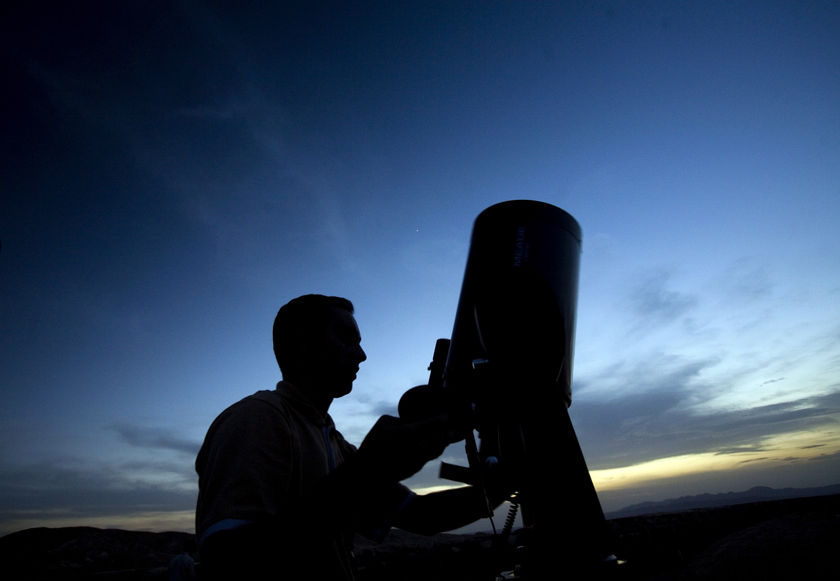
\includegraphics[scale=0.69]{graphics/Astronomer.jpg}\cite{pic_astronomer}	
		\end{column}}{}
		
		\alt<2>{\begin{column}{\textwidth}
			\centering 
			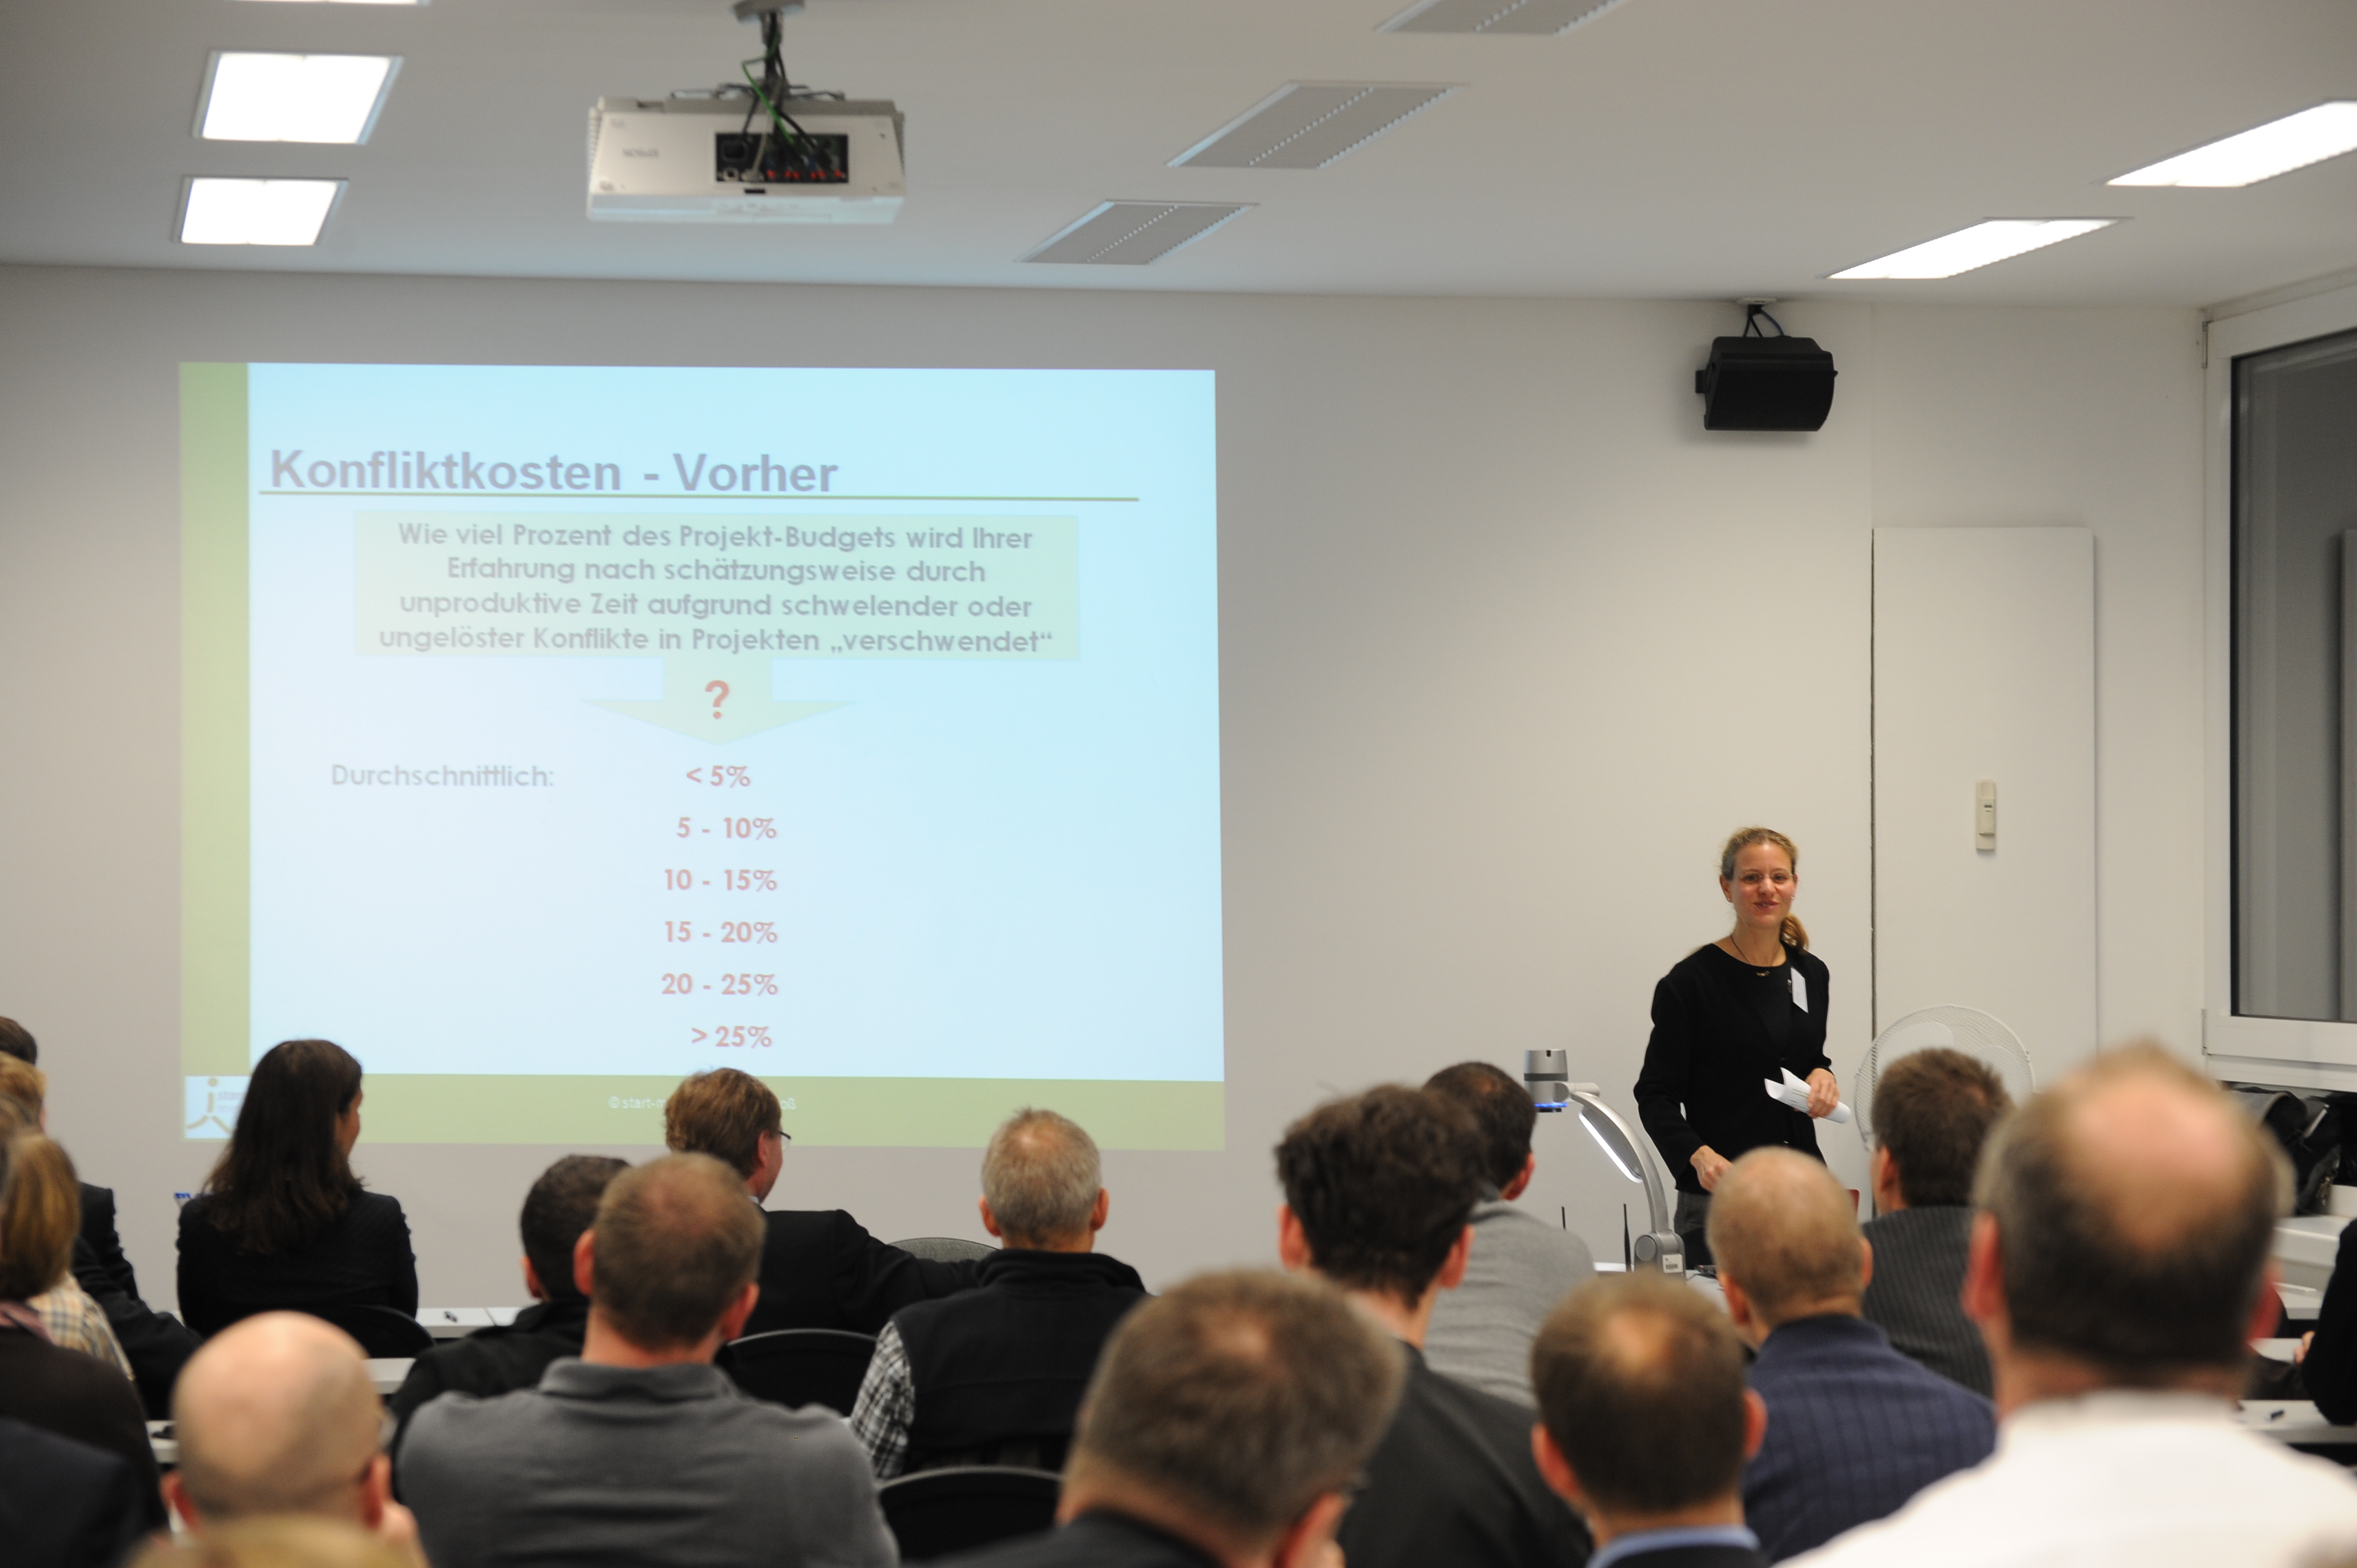
\includegraphics[scale=0.145]{graphics/Vortrag_PMI.jpg}\cite{pic_presentation}
		\end{column}}{}
	\end{columns}
\end{frame}
		\begin{frame}{Bewusstsein}
	\only<1>{Definition Duden\,\cite{duden_consciousness}:
	\begin{itemize}
		   \item{\Quote{Zustand, in dem man sich einer Sache bewusst ist; deutliches Wissen von etwas, Gewissheit}}
		   \item{\Quote{Gesamtheit der Überzeugungen eines Menschen, die von ihm bewusst vertreten werden}}
		    \item{\Quote{(Psychologie) Gesamtheit aller jener psychischen Vorgänge, durch die sich der Mensch der Außenwelt und seiner selbst bewusst wird}}
		   \item{\Quote{Zustand geistiger Klarheit; volle Herrschaft über seine Sinne}}
	\end{itemize}}
	
	\only<2->{\begin{itemize}
			\item{Duden: \Quote{(Psychologie) Gesamtheit aller jener psychischen Vorgänge, durch die sich der Mensch der Außenwelt und seiner selbst bewusst wird}\,\cite{duden_consciousness}}
			\item{Allgemein: Subjektiv, nicht fassbar nur erfahrbar}
			\item{\emph{Das schwierige Problem}: Warum nehmen wir wahr?}
			\begin{quote}
				\enquote{What is your extra ingredient, and why should that account for conscious experience?}
				- David Chalmers\,\cite{Chalmers_95} 
			\end{quote}
			\item{Häufige Antwort: Dualismus}
				\begin{itemize}
					\item{physische Materie} 
					\item{nicht-physische \enquote{Lebenskraft} (Seele)}
				\end{itemize}
	\end{itemize}}
\end{frame}
	
	\section{Betrachtung und Probleme in der Physik}
		\separatorslide
		\begin{frame}{Beobachter}
	\begin{itemize}
		\item{Definition abhängig von Betätigungsfeld}
		\item{Allgemeine Relativitätstheorie:}
		\begin{itemize}
			\item{keine Masse oder Ausdehnung}
			\item{keinen Einfluss auf das Beobachtete}
		\end{itemize}
		\item{Quantenmechanik:}
		\begin{itemize}
			\item{Einfluss: Kollaps/Branching der Wellenfunktion}
		\end{itemize}
		\item{\Quote{The only issue there is consensus on is that there is no
				consensus about how to define an observer and its role.}\\ - Max Tegmark\,\cite{Tegmark_15_long}}
	\end{itemize}
\end{frame}
		\begin{frame}{Bewusstsein}
	\begin{itemize}
		\item{im allgemeinen unbeachtet}
		\begin{itemize}
			\item{\Quote{ An other argument physics has been managed just fine for hundreds of years avoiding this subject and should therefore keep doing so.} - Max Tegmark\,\cite{Tegmark_15_long}}
%			\item{\Quote{A commonly held view is that consciousness is irrelevant to physics and should therefore not be discussed in physics papers.}\\ - Max Tegmark\,\cite{Tegmark_15_long}}
		\end{itemize}
		\item{keine Lösung für \emph{schwieriges Problem}}
		\begin{itemize}
			\item{Dualismus nur schwer zu vertreten}
			\end{itemize}
		\item{Einfluss von respektive auf Quantenmechanik unklar}
		\begin{itemize}
			\item{Gehirn: nass und warm }
		\end{itemize}
	\end{itemize}
\end{frame}
		
	\section{Beobachter als Teilsystem}
		\separatorslide
		\begin{frame}{Beobachter als Teilsystem}
	\begin{itemize}
		\item{Zerlegung eines Systems beschreiben durch $H$ und $\rho$}
	\end{itemize}
	\begin{beamerboxesrounded}{3 Teilsysteme + Wechselwirkung}
		\begin{empheq}{align*}
		H &= H_{\mathrm{O}} + H_{\mathrm{E}} + H_{\mathrm{S}} + H_{\mathrm{int}}\\
		H_{\mathrm{int}} &= H_{\mathrm{OE}} + H_{\mathrm{ES}} + H_{\mathrm{OS}} + H_{\mathrm{OES}}
		\end{empheq}
		\vspace{-0.5cm}
	\end{beamerboxesrounded} 
	\begin{itemize}
		\item{Subjekt (S): Freiheitsgrade der subjektiven Wahrnehmung des Beobachters}
		\item{Objekt (O): Zu beobachtende Freiheitsgrade}
		\item{Umgebung (E): Alle übrigen Freiheitsgrade des Systems}
	\end{itemize}
\end{frame}

		\begin{frame}{Beispiel: $H_{\mathrm{O}}$, $H_{\mathrm{OE}}$, $H_{\mathrm{OS}}$}
	\alt<1>{\begin{itemize}
		\item{Betrachtung mit je einem Freiheitsgrad für (S) und (O)}
		\begin{itemize}
			\item{Subjekt: \ketsmiley, \ketneutrey, \ketfrowny}
			\item{Objekt: \ketup, \ketdown}
		\end{itemize}
		\item{Gesamtsystem S $\otimes$ O mit 6 Basiszuständen:\\
			\ketsmileyup, \ketsmileydown,\ketneutreyup, \ketneutreydown,\ketfrownyup, \ketfrownydown}
		\item{Dichtematrix $\rho = \ketneutreyup\braneutreyup$ als Anfangszustand:\\}
			\vspace{0.2cm}
			\centering
			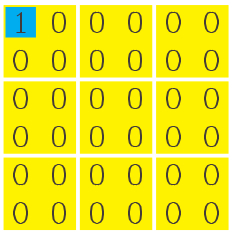
\includegraphics[scale=0.3]{graphics/subsystem_example_1_1.jpg}
	\end{itemize}}{}
		\alt<2>{\begin{itemize}
				\item{Zeitentwicklung $U = \exp(-i H_{\mathrm{O}}t)$ von $\rho_{\mathrm{O}} = \ketup\braup$}
				\begin{itemize}
					\item{$U\ketup = \frac{1}{\sqrt{2}}\del{\ketup + \ketdown}$}
					\item{Entropie bleibt konstant}
				\end{itemize}
				\end{itemize}
				\begin{columns}
					\begin{column}{0.55\textwidth}
						\begin{beamerboxesrounded}{}
							\begin{align*}
							\rho^{\prime}_{\mathrm{O}} = U\rho_{\mathrm{O}}U^{\dagger}
							=&\frac{1}{2}(\ketup\braup + \ketup\bradown \\ &+ \ketdown\braup + \ketdown\bradown)
							\end{align*}
							\vspace{-0.5cm}
						\end{beamerboxesrounded}
					\end{column}
					\begin{column}{0.35\textwidth}
						 \centering
						 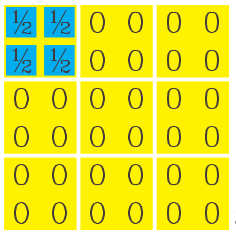
\includegraphics[scale=0.35]{graphics/subsystem_example_1_2.jpg}
					\end{column}
				\end{columns}}{}
				
		\alt<3>{\begin{itemize}
				\item{$H_{\mathrm{OE}}$: Dekohärenz (vollständig)}
				\begin{itemize}
					\item{Entropie nimmt zu}
				\end{itemize}
				\vspace{0.2cm}
				%				\centering
				%				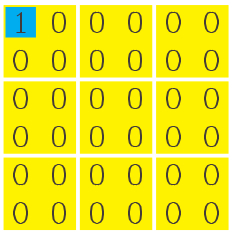
\includegraphics[scale=0.3]{graphics/subsystem_example_1_1.jpg}
			\end{itemize}
			\begin{columns}
				\begin{column}{0.55\textwidth}
					\begin{beamerboxesrounded}{}
						\begin{equation*}
						\rho^{\prime\prime}_{\mathrm{O}} = \frac{1}{2}(\ketup\braup + \ketdown\bradown)
						\end{equation*}
						\vspace{-0.5cm}
					\end{beamerboxesrounded}
				\end{column}
				\begin{column}{0.35\textwidth}
					\centering
					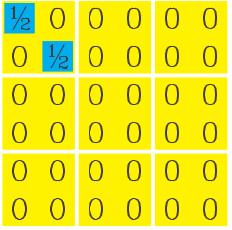
\includegraphics[scale=0.35]{graphics/subsystem_example_1_3.jpg}
				\end{column}
			\end{columns}}{}
		\alt<4>{\begin{itemize}
				\item{$H_{\mathrm{OS}}$: Messung von S an O}
				\begin{itemize}
					\item{$U = \exp(-i \int\!\!\!H_{\mathrm{OS}}\dif t)$, Messung schnell}
					\item{$U\ketneutreyup = \ketsmileyup$, $U\ketneutreydown = \ketfrownydown$}
					\item{$\rho_{\mathrm{OS}} = \ketneutrey\braneutrey \otimes \frac{1}{2}(\ketup\braup + \ketdown\bradown)$}
					\item{Entropie nimmt ab}
				\end{itemize}
				\vspace{0.2cm}
				%				\centering
				%				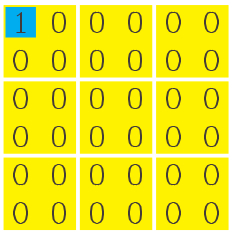
\includegraphics[scale=0.3]{graphics/subsystem_example_1_1.jpg}
			\end{itemize}
			\begin{columns}
				\begin{column}{0.55\textwidth}
					\begin{beamerboxesrounded}{}
						\begin{empheq}{align*}
						\rho^{\prime}_{\mathrm{OS}} = U\rho_{\mathrm{OS}}U^{\dagger} = &\frac{1}{2}(\ketsmileyup\brasmileyup\\ &+ \ketfrownydown\brafrownydown)
						\end{empheq}
						\vspace{-0.5cm}
					\end{beamerboxesrounded}
				\end{column}
				\begin{column}{0.35\textwidth}
					\centering
					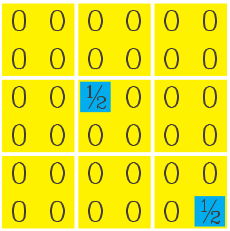
\includegraphics[scale=0.35]{graphics/subsystem_example_1_4.jpg}
				\end{column}
			\end{columns}}{}
%			\alt<5>{\begin{columns}
%					\begin{column}{0.45\textwidth}
%						\centering
%						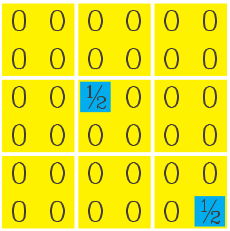
\includegraphics[scale=0.35]{graphics/subsystem_example_1_4.jpg}
%					\end{column}
%					\begin{column}{0.45\textwidth}
%						\centering
%						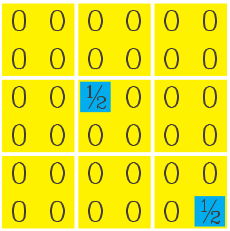
\includegraphics[scale=0.35]{graphics/subsystem_example_1_4.jpg}
%					\end{column}
%				\end{columns}}{}}{}		
\end{frame}
		\begin{frame}{Beispiel: $H_{\mathrm{S}}$, $H_{\mathrm{SE}}$}
	\alt<1,2>{\begin{itemize}
		\item{Zeitentwicklung von S}
		\begin{itemize}
			\item{$U = \exp(-i \int\!\!\!H_{\mathrm{OS}}\dif t)$, spontane Entscheidung}
			\item{$U\ketneutrey = \frac{1}{\sqrt{2}}\del{\ketsmiley + \ketfrowny}$, $\rho_{\mathrm{S}} = \ketneutrey\braneutrey$}
		\end{itemize}
	\end{itemize}
				\begin{columns}
					 \alt<1>{\begin{column}{\textwidth}
					 	\vspace{0.25cm}
		 			 	\centering
		 			 	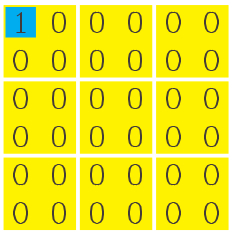
\includegraphics[scale=0.35]{graphics/subsystem_example_1_1.jpg}
					 	\end{column}}{}
					\alt<2>{\begin{column}{0.55\textwidth}
						\begin{beamerboxesrounded}{}
							\begin{align*}
							\rho^{\prime}_{\mathrm{S}} = U\rho_{\mathrm{S}}U^{\dagger}
							=&\frac{1}{2}(\ketsmiley\brasmiley + \ketsmiley\brafrowny \\ &+ \ketfrowny\brasmiley + \ketfrowny\brafrowny)
							\end{align*}
							\vspace{-0.5cm}
						\end{beamerboxesrounded}
					\end{column}
					\begin{column}{0.35\textwidth}
						 \centering
						 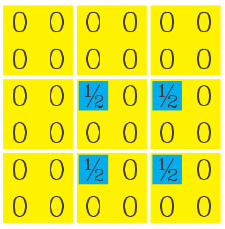
\includegraphics[scale=0.35]{graphics/subsystem_example_2_2.jpg}
					\end{column}}{}
				\end{columns}}{}	
	\alt<3>{\begin{itemize}
			\item{$H_{\mathrm{SE}}$: Dekohärenz des Subjekts}
		\end{itemize}
		\begin{columns}
			\begin{column}{0.55\textwidth}
				\begin{beamerboxesrounded}{}
					\begin{equation*}
					\rho^{\prime\prime}_{\mathrm{S}} = \frac{1}{2}(\ketsmiley\brasmiley + \ketfrowny\brafrowny)
					\end{equation*}
					\vspace{-0.5cm}
				\end{beamerboxesrounded}
			\end{column}
			\begin{column}{0.35\textwidth}
				\centering
				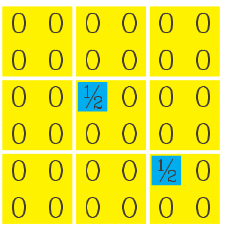
\includegraphics[scale=0.35]{graphics/subsystem_example_2_3.jpg}
			\end{column}
		\end{columns}
	\begin{itemize}
		\item{Auf welchen Zeitskalen läuft Dekohärenz im Gehirn ab?}
	\end{itemize}}{}			
		
\end{frame}
		\begin{frame}{Implikationen dieses Modells}
	\begin{itemize}
		\item{Prämisse: Freiheitsgrade des Subjekts sind die Wahrnehmungen des Beobachters}
		\item{Hohe Korrelation zu einer Auswahl von Eigenschaften der Umgebung und des Objekts}
		\begin{itemize}
			\item{Aufnahme von Reizen durch Sinnesorgane}
			\item{Korrelation zu vergangenen Zuständen}
		\end{itemize}
		\item{Transinformation zwischen Subjekt und Objekt + Umgebung relativ konstant}
			\begin{itemize}
					\item{Information über Umwelt durch Sinne}
					\item{Zunahme durch Lernen, Abnahme durch Vergessen}
			\end{itemize}
	\end{itemize}
\end{frame}
		
		
	\section{Dekohärenz von Gehirnprozessen}
		\separatorslide
		\begin{frame}{Superposition von Neuronen}
\begin{columns}
		\alt<1>{\begin{column}{0.55\textwidth}
			\begin{itemize}
				\item{Neuronen: Bausteine des menschlichen Gehirns \textasciitilde $10^{11}$}
				\begin{itemize}
					\item{komplexes Netzwerk}
					\item{Verbindung mit dem Bewusstsein anzunehmen}
				\end{itemize}
				\item{Zwei mögliche Zustände}	
				\begin{itemize}
					\item{feuern $\leftrightarrow$ nicht feuern}
				\end{itemize}
			\end{itemize}
		\end{column}
		\begin{column}{0.4\textwidth}
			\centering
			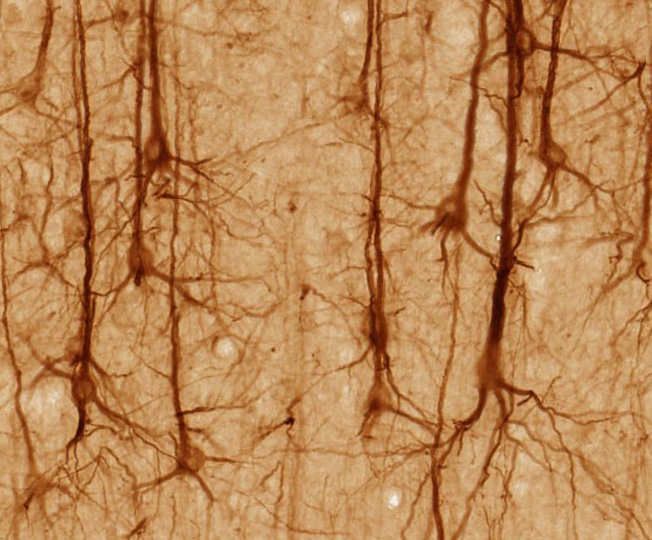
\includegraphics[scale=0.8]{graphics/neuron.jpg}\,\cite{neurons}
		\end{column}}{}
		\alt<2>{\begin{column}{0.45\textwidth}
			\begin{itemize}
				\item{Einfache Annahmen}
				\begin{beamerboxesrounded}{Anzahl der Na$^{\textcolor{white}{+}}$-Ionen}
					\begin{empheq}{equation*}
						N = \frac{\pi dLf\epsilon_{0}}{qh}\del{U_{1} -U_{0}}
					\end{empheq}
					\vspace{-0.5cm}
				\end{beamerboxesrounded}	

			\item{$h=\SI{8}{nm}$, $d=\SI{10}{\micro\metre}$,\\ $L=\SI{10}{\centi\metre}$, $f=\num{e-3}$,\\
				  $U_{0} = \SI{-0.07}{\volt}$, $U_{1} = \SI{0.03}{\volt}$}
				\begin{itemize}
					\item{$N \sim \num{e6}$}
				\end{itemize}
			\end{itemize}
		\end{column}
		\begin{column}{0.45\textwidth}
			\centering
			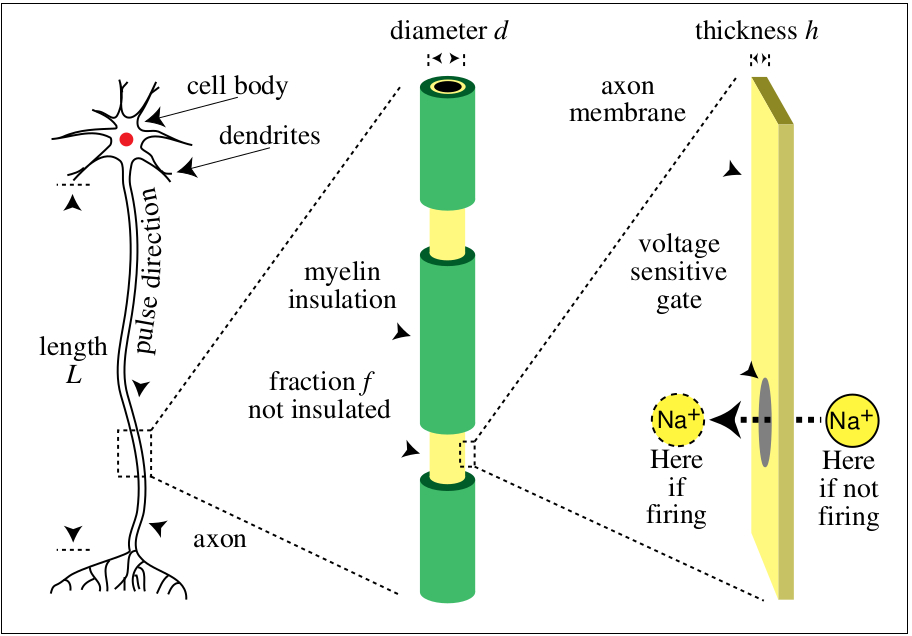
\includegraphics[scale=0.18]{graphics/neuron_schematic.jpg}\\\hfill\cite{Tegmark_99}
		\end{column}}{}
	\end{columns}	
	\alt<2>{\begin{itemize}
		\item[$\Rightarrow$]{Räumliche Superposition von \num{e6} Na$^{+}$-Ionen, mit Abstand  $\sim\mathcal{O}(\SI{10}{nm})$}
	\end{itemize}}{}
\end{frame}
		\begin{frame}{Dekohärenz von Neuronen}
	\alt<1>{\begin{itemize}
		\item{Unterschiedliche Wechselwirkungen}
		\begin{itemize}
			\item{Stöße zwischen Na$^{+}$-Ionen, anderen Ionen und H$_{2}$O-Molekülen }
			\item{Coulombabstoßung der Na$^{+}$ von andern Ionen}
		\end{itemize}
		\item{Abschätzung der Größenordnung, unteres Limit}
		\item{Coulombabstoßung: nächstes Ion größter Beitrag}
		\item{Stoßprozesse dekohärieren Ion auf de-Broglie Wellenlänge des Stoßteilchens}
	\end{itemize}}{}
	\alt<2,3>{\begin{itemize}
			\item{Betrachtete Wechselwirkungen liefern}
		\end{itemize}
			\begin{beamerboxesrounded}{Zeitentwicklung von $\textcolor{white}{\rho}$}
				\begin{empheq}{equation*}
					\rho(x, x^{\prime},t_{0}+t) = \rho(x, x^{\prime},t_{0}) f(x,x^{\prime},t)
				\end{empheq}
				\vspace{-0.5cm}
			\end{beamerboxesrounded}
			\begin{itemize}
			\alt<2>{\item{Ergebnisse für Dekohärenz-Zeitskalen}}{\item{Mikrotubuli}}
			\begin{columns}
%				\begin{column}{.05\textwidth}
%					\hfill
%				\end{column}
				\only<2>{\begin{column}{\textwidth}
					\centering
					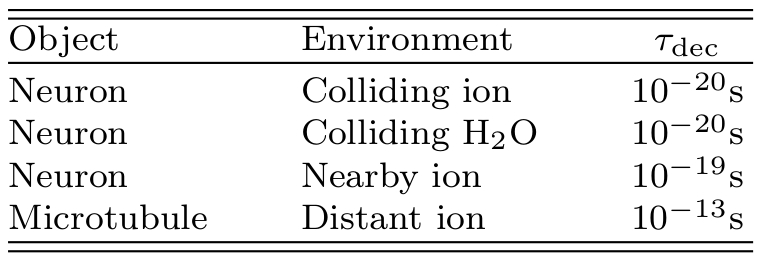
\includegraphics[scale=0.23]{graphics/decoherance_timescales.jpg}\,\cite{Tegmark_99}
				\end{column}}	
				\only<3>{\begin{column}{.45\textwidth}
					\centering
					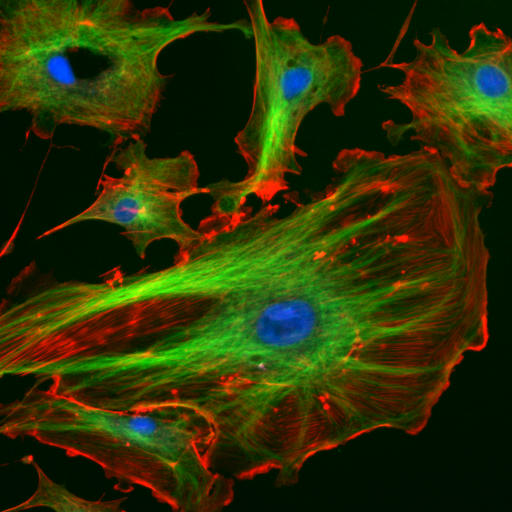
\includegraphics[scale=0.2]{graphics/FluorescentCells.jpg}\,\cite{microtubule}
				\end{column}
				\begin{column}{.55\textwidth}
					\centering
					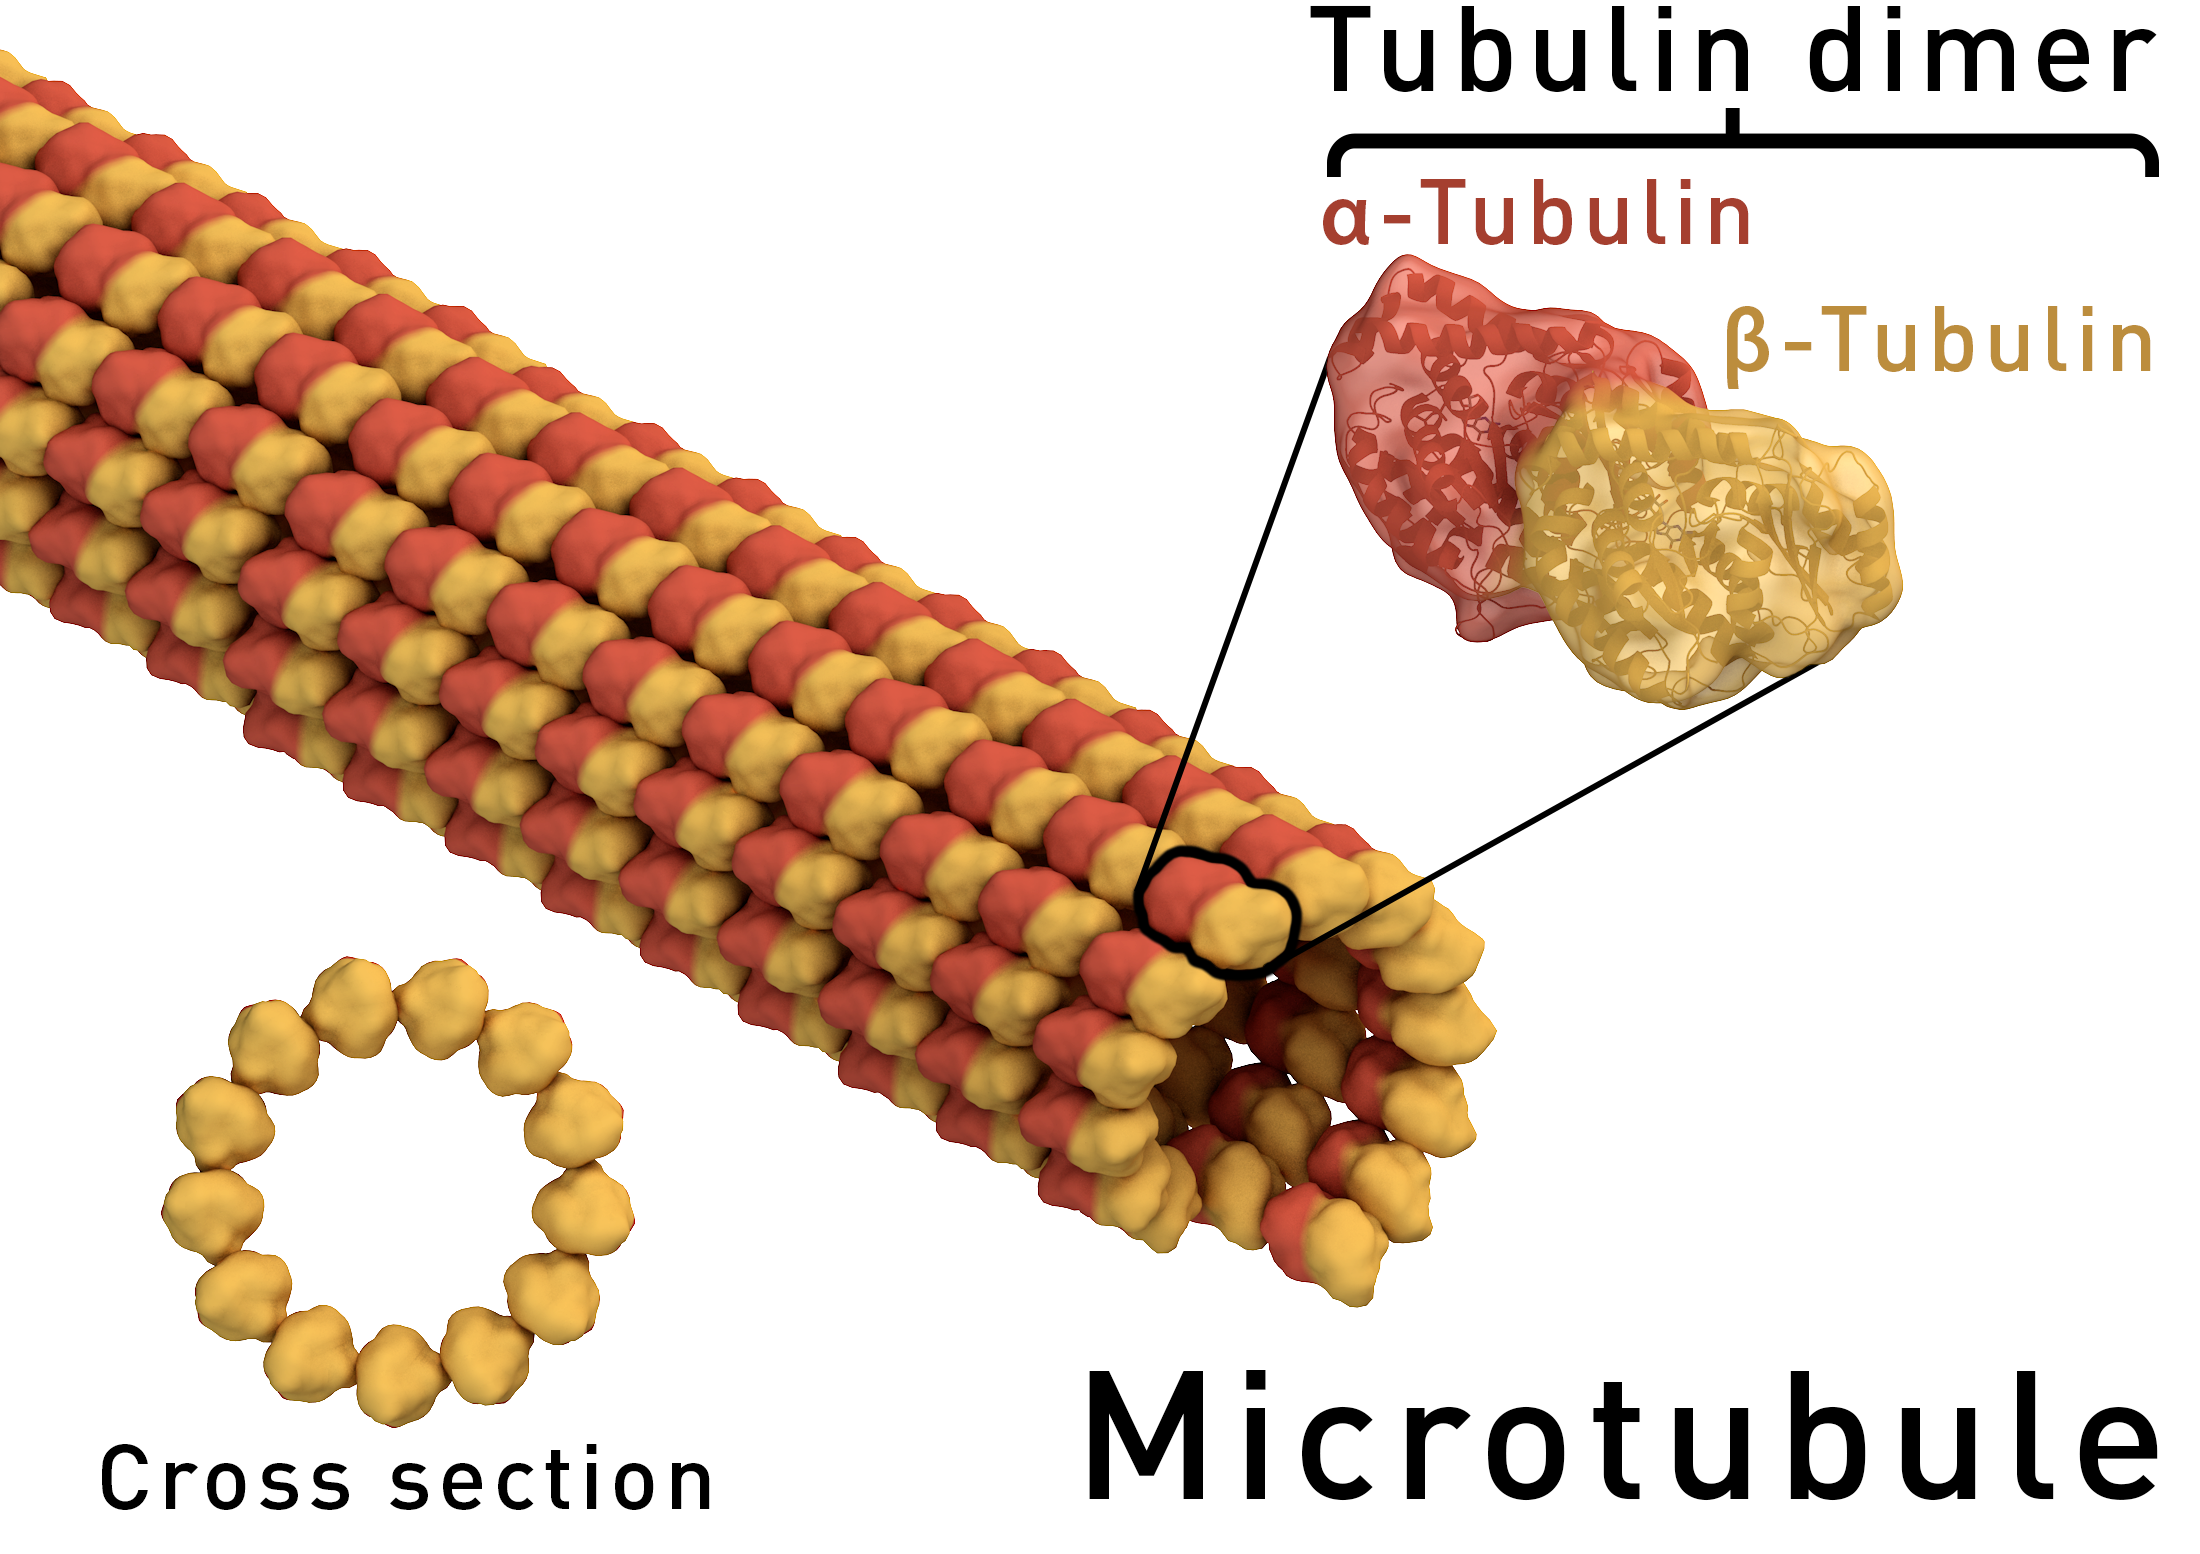
\includegraphics[scale=0.07]{graphics/Microtubule_structure.png}\,\cite{microtubule_structure}
			\end{column}}						
			\end{columns}
		 \alt<2>{\item{typische Dynamik-Zeitskalen sind $(\num{e-4} \text{ -- } 10^{0})\si{\second}$}
		 \begin{itemize}
		 	\item{Dekohärenz zerstört Superpositionen\\ schon bei der Entstehung}
		 	\item{Hirnprozesse als klassisch zu betrachten}
		 \end{itemize}}{}
		\end{itemize}}{}
\end{frame}
				
	\section{Bewusstsein als Aggregatzustand}
		\separatorslide
		\begin{frame}{Bewusstsein als Aggregatzustand}
	\begin{columns}
		\begin{column}{0.55\textwidth}
			\begin{itemize}
				\item{Aggregatzustände durch Eigenschaften unterscheidbar}
				\item{Ähnliche Konzepte bereits erdacht}
				\begin{itemize}
					\item{\emph{Computronium}}
				\end{itemize}
				\item{Welche Eigenschaften muss \emph{Perceptronium} besitzen?}
			\end{itemize}
		\end{column}
		\begin{column}{0.45\textwidth}
			\centering
			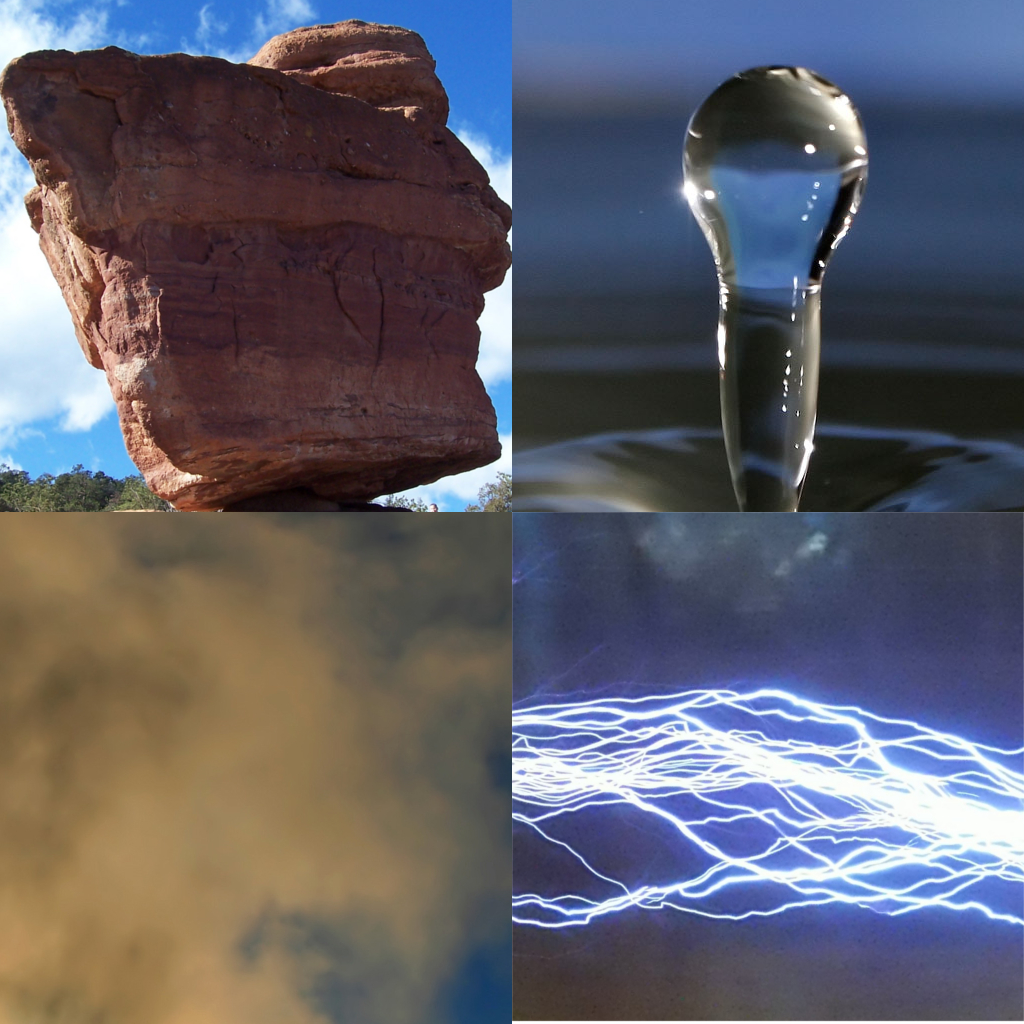
\includegraphics[scale=0.15]{graphics/states_of_matter.jpg}\\\hfill\cite{pic_stone,pic_water_droplet,steam_eruption,lightning_teslacoil}
		\end{column}
	\end{columns}
\end{frame}
		\begin{frame}{Eigenschaften von Perceptronium}
	\begin{itemize}
		\item{Aktive Forschung z.B. in der Neurowissenschaft}
		\begin{itemize}
			\item{G. Tononi (\textsc{Integrated Information Theory})\,\cite{Tononi_08}}
  		\end{itemize}
	\end{itemize}
	\begin{beamerboxesrounded}{Integrierte Information $\textcolor{white}{\Phi}$ (abgewandelt)}
		\begin{empheq}{equation*}
			\Phi = I_{\mathrm{min}} = \min_{\rho_1,\rho_2} \del{S(\rho_{1}) + S(\rho_{2}) - S(\rho)}
		\end{empheq}
		\vspace{-0.5cm}
		\begin{empheq}{equation*}
			\small I: \text{Transinformation}, S = - \Tr[\rho\log_{2}(\rho)]
		\end{empheq}
		\vspace{-0.5cm}
	\end{beamerboxesrounded}
	\begin{itemize}
		\item{Minimale Transinformation nach einem Schnitt der das System in zwei teilt}
			\begin{itemize}
				\item{\Quote{the cruelest cut} - Giulio Tononi}
				\item{Maximale Unabhängigkeit der Teilsysteme,\\ $\Phi = 0 \Leftrightarrow$ vollständig unabhängig}
			\end{itemize}
	\end{itemize}
\end{frame}
		\begin{frame}{Integrierte Information}
		\begin{columns}
			\alt<1,2>{\begin{column}{0.55\textwidth}
				\begin{itemize}
					\item{Betrachtbar als Speicherung von Information,
						mit Fehlerkorrektur-Mechanismus}
					\item{Integrierte Information für $k$ zufällig ausgewählte
						  14-bit-Folgen}
					\begin{itemize}
						\item{Maximum bei $k \approx 2^{7}$}
					\end{itemize}
				\end{itemize}
			\end{column}
			\begin{column}{0.5\textwidth}
				\centering
				\alt<1>{
\includegraphics[scale=0.14]{graphics/qrcode_whole.jpg}}{}
				\alt<2>{\hspace{-0.08cm}
\includegraphics[scale=0.14]{graphics/qrcode_damaged.jpg}}{}
			\end{column}}{}

		\alt<3>{\begin{column}{0.55\textwidth}
				\begin{itemize}
					\item{Physikalische Systeme}
					\begin{itemize}
						\item{\enquote{Eierkarton}-Potential ($16\times16$)}
						\item{Oben 256 Minima, $S(\text{Grundzustand}) = 8$}
						\item{Unten 16 Minima, $S(\text{Grundzustand}) = 4$}
					\end{itemize}
					\item{Ort $\del{x,y}$ als zwei 4-bit Zahlen: $0_{2} \text{ -- } 15_{2}$}
					\item{Integration}
						\begin{itemize}
							\item{Oben schlecht $\Phi = 0$}
							\item{Unten gut $\Phi = 2$}
						\end{itemize}
				\end{itemize}
			\end{column}
			\begin{column}{0.5\textwidth}
				\centering
				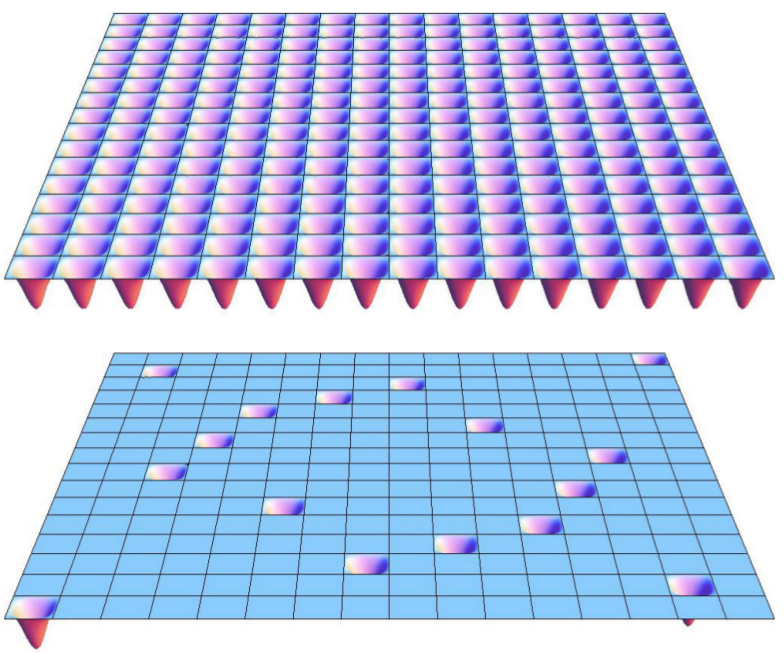
\includegraphics[scale=0.18]{graphics/egg_crate_potentials.jpg}\,\cite{Tegmark_15_long}
			\end{column}}{}	
		\end{columns}
			\centering
			\alt<1,2>{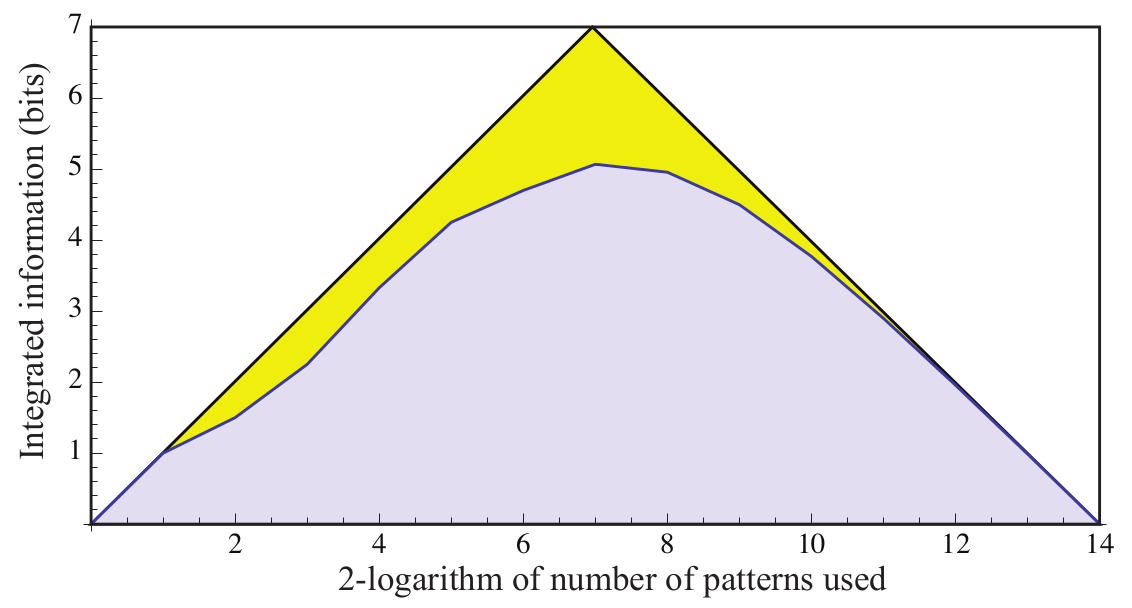
\includegraphics[scale=0.16]{graphics/integrated_information_graph.jpg}\cite{Tegmark_15_long}}{}
\end{frame}
		\begin{frame}{Probleme mit Integration}
	\begin{itemize}
		\item{Informationsgehalt des Zustand $\rho$ und des Systems $H$}
	\end{itemize}
		\begin{beamerboxesrounded}{\enquote{Eierkarton} -Potential mit $\textcolor{white}{k}$ Minima}
			\begin{empheq}{equation*}
			S(\rho) \sim \log_{2}(\text{\# möglicher Zustände}) \sim n
			\end{empheq}
			\vspace{-0.5cm}
			\begin{empheq}{equation*}
			S(H) \sim \log_{2}(\text{\# möglicher } H) \sim kn
			\end{empheq}
			\vspace{-0.5cm}
			\end{beamerboxesrounded}
	\begin{itemize}
		\item{Gehirn mit \num{e11} Neuronen}
	\end{itemize}
				\begin{beamerboxesrounded}{Maximale Integration}
					\begin{empheq}{equation*}
					S(H) \sim \sqrt{2^{n}}\frac{n}{2} \sim 10^{10^{10}} \text{bit}
					\end{empheq}
					\vspace{-0.5cm}
				\end{beamerboxesrounded}
		\begin{itemize}
			\item{Notwendige Dynamik viel zu komplex}
		\end{itemize}
\end{frame}
		\begin{frame}{Eigenschaften von Perceptronium}
	\centering
	\only<1>{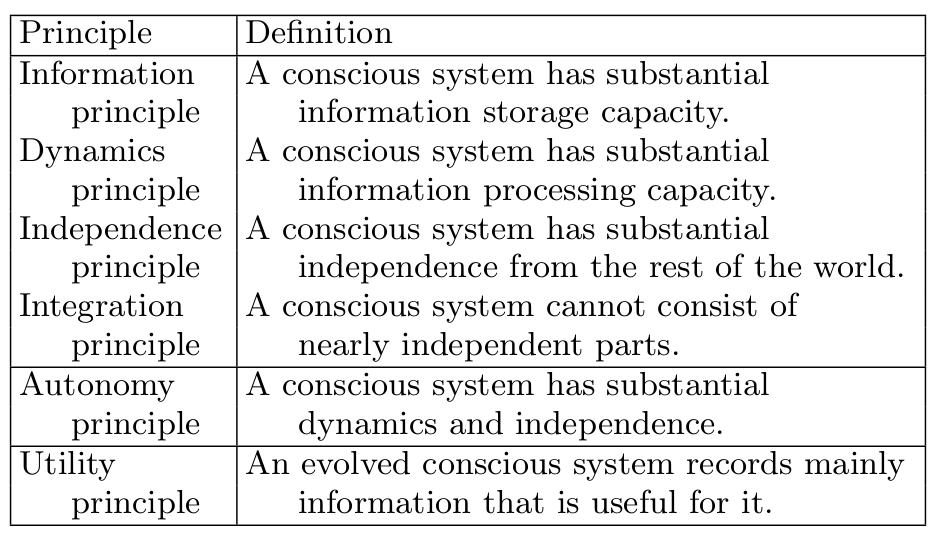
\includegraphics[scale=0.3]{graphics/property_principles.jpg}\,\cite{Tegmark_15_long}}
	\only<2>{\hspace{-0.08cm}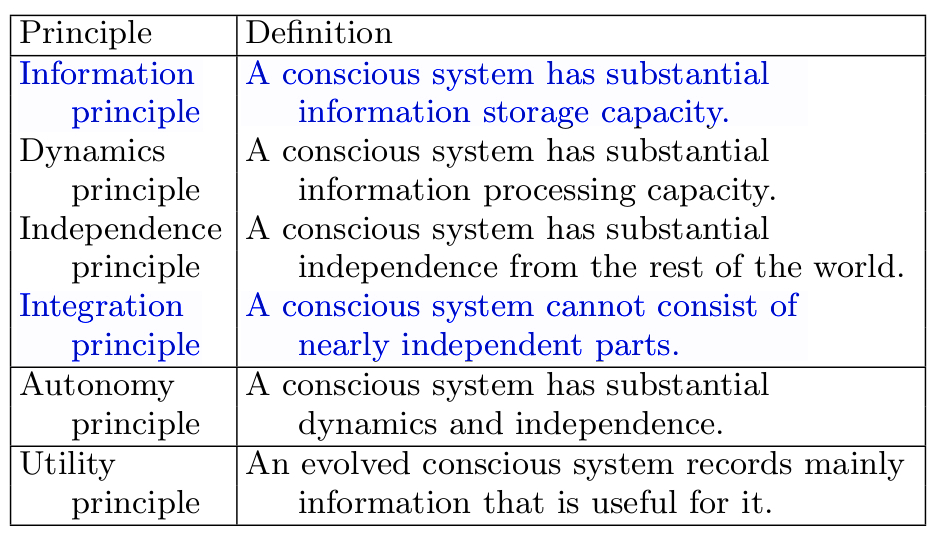
\includegraphics[scale=0.3]{graphics/property_principles_1.jpg}\,\cite{Tegmark_15_long}}
%	\only<3>{\hspace{-0.16cm}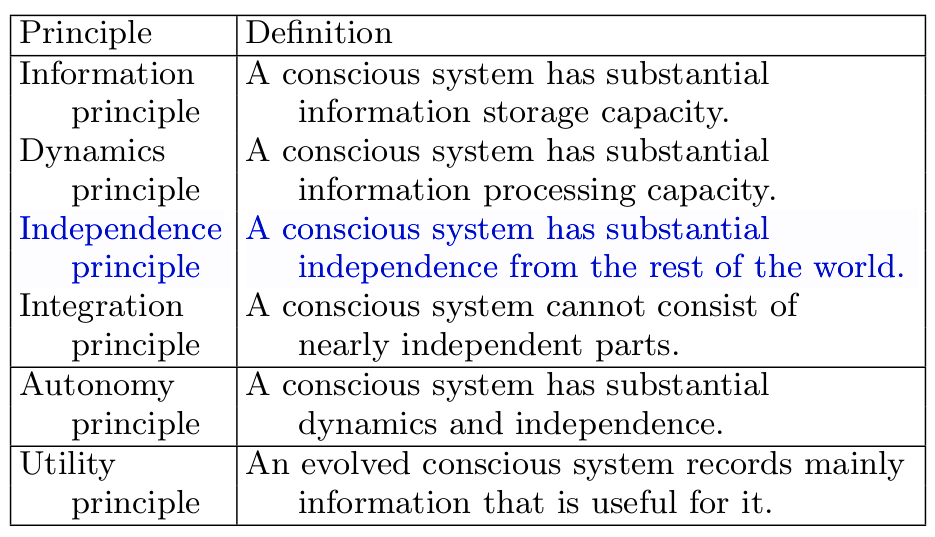
\includegraphics[scale=0.3]{graphics/property_principles_2.jpg}\,\cite{Tegmark_15_long}}
	%\only<4>{\hspace{-0.24cm}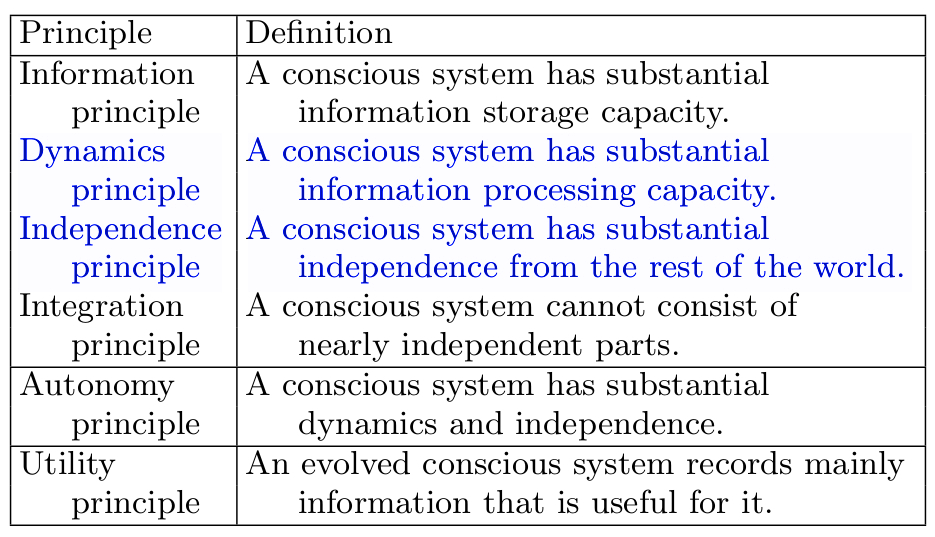
\includegraphics[scale=0.3]{graphics/property_principles_3.jpg}\,\cite{Tegmark_15_long}}
	%\only<5>{\hspace{-0.32cm}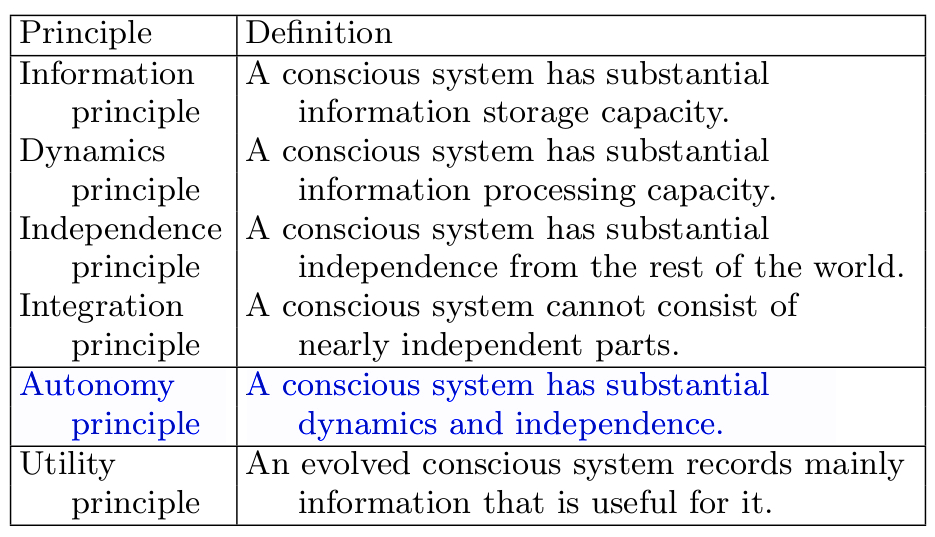
\includegraphics[scale=0.3]{graphics/property_principles_4.jpg}\,\cite{Tegmark_15_long}}
\end{frame}
		\begin{frame}{Unabhängigkeit}
	\begin{columns}
		\alt<1>{\begin{column}{0.55\textwidth}
			\begin{itemize}
				\item{Als Maß für Unabhängigkeit wiederum $\Phi$ verwendbar}
				\item{klassisches 2-bit-System, {\footnotesize$\rho = \begin{pmatrix} P(\downarrow\downarrow) & P(\downarrow\uparrow)\\P(\uparrow\downarrow) & P(\uparrow\uparrow)\end{pmatrix}$}}
				\begin{itemize}
					\item{nur ein Schnitt in zwei einzelne bits möglich $\Rightarrow \Phi = I$}
					\item{helles Dreieck}
				\end{itemize}
				\item{2-qbit-System: $\rho \in \mathbb{R}^{4\times4}$}
				\begin{itemize}
					\item{zusätzlich dunkles Dreieck}
					\item{$\Phi = \displaystyle\min_{U} I\del{U\rho U^{\dagger}}$}
				\end{itemize}
			\end{itemize}		
		\end{column}}{}
		\alt<2>{\begin{column}{0.55\textwidth}
				\begin{itemize}
					\item{Bell-Paar (4): $\ket{\Psi} = \frac{1}{\sqrt{2}} \del{\ketup\!\ketup + \ketdown\!\ketdown}$  }
					\begin{itemize}
						\item{Reiner Zustand,\\ Trafo $\Rightarrow$ $\rho = \ketup\!\braup$}
						\item{separabel $\Rightarrow \Phi = 0$}
					\end{itemize}
					\item{maximale Verschränkung, keine Integrierte Information}
					\begin{itemize}
						\item{\Quote{the \textbf{cruelest} cut}}
					\end{itemize}
				\end{itemize}		
			\end{column}}{}
		
		\begin{column}{0.55\textwidth}
			\centering
			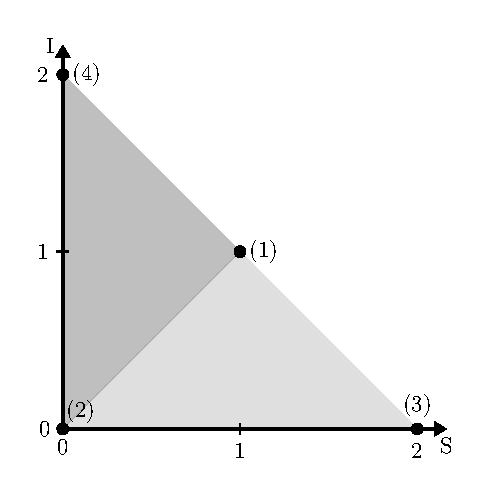
\includegraphics[scale=0.65]{graphics/presentation_qm.pdf}\,\cite{Tegmark_15_long}
			\footnotesize
			(1): $\rho = \frac{1}{2} \del{\ketup\!\braup + \ketdown\!\bradown}$\\
			\hspace{-1.65cm}(2): $\rho = \ketup\!\braup$\\
			\hspace{-.2cm}(3): $\rho = \frac{1}{4} (\ketup\!\braup + \ketdown\!\braup$\\\qquad\qquad $+ \ketup\!\bradown + \ketdown\!\bradown)$\\
			(4): $\rho = \frac{1}{2} \del{\ketup\!\ketup + \ketdown\!\ketdown}$ \\\qquad\qquad$\del{\braup\!\braup + \bradown\!\bradown} $\\
		\end{column}		
	\end{columns}
\end{frame}
		%TODO: Wort auswählen
\begin{frame}{Unabhängigkeit von Quantenzuständen}
	\begin{itemize}
		\item{Bell-Paar und perfekt korrelierte klassische bits,
			  keine integrierte Information}
		\begin{itemize}
			\item{Wie hoch kann $\Phi$ quantenmechanisch werden?}
		\end{itemize}
	\end{itemize}
	\begin{beamerboxesrounded}{$\textcolor{white}{\rho}$-Diagonalitäts-Satz}
		Die Transinformation $I$ ist in einer Basis am geringsten,\\ in der $\rho$
		diagonal ist.
	\end{beamerboxesrounded}
		\begin{itemize}
			\item{für $\rho \in \mathbb{R}^{4\times4}$ mit $n$ nicht entarteten Eigenwerten,\\
				Diskrete Minimierung über $n!$ Permutationen}
			\begin{itemize}
				\item{höhste Werte für $\Phi$ bei $\rho \propto \rho^{2}$,
					  $k$ Eigenwerte sind $k^{-1}$ übrige sind 0}
				\item{$n=4, k=3 \Rightarrow \Phi \approx \num{0.2516}$ bit}
			\end{itemize}
			\item{klassische: $\Phi = \mathcal{O}(n)$,\\ quantenmechanisch: $n \to \infty \Rightarrow \Phi \to 0$  }
		\end{itemize}
\end{frame}
		\begin{frame}{Unabhängigkeit von Quantensytemen}
	\alt<1>{\begin{itemize}
		\item{Allgemeiner Hamiltonoperator $H$}
	\end{itemize}
	\begin{beamerboxesrounded}{Separation in Teilsysteme und Wechselwirkung}
		\begin{empheq}{equation*}
			H = H_{1} \otimes I  +  I \otimes H_{2} + H_{3}
		\end{empheq}
		\vspace{-0.5cm}
	\end{beamerboxesrounded}
		\begin{itemize}
			\item{$H_{3} = 0$: $H_{1},H_{2}$ \enquote{parallele Universen}}
					\begin{itemize}
						\item{der härteste Schnitt bei minimalem $H_{3}$}
					\end{itemize}
		\end{itemize}}{}	
	\alt<1,2>{\begin{beamerboxesrounded}{$\textcolor{white}{H}$-Diagonalitäts-Satz}
			Der Hamiltonoperator $H$ ist immer in der Energieeigenbasis, in der $H$ diagonal ist maximal separierbar 
			( $\norm{H_3}$ minimal).
	\end{beamerboxesrounded}}{}
	\alt<2>{\begin{itemize}
			\item{In dieser Separation kommutieren $H_1$ und $H_2$ mit einander und mit $H_3$}
			\begin{itemize}
				\item{ähnlich zur Zeiger-Basis von Zurek, Zustände kommutieren mit 
					WW-Hamiltonoperator\,\cite{Zurek_01}}
			\end{itemize}
		\end{itemize}}{}
		\alt<2,3>{\begin{itemize}
				\item{Dekohärenz treibt System $H_1$ mit $\comm{H_1}{H_3} = 0$ in einen zeitunabhängigen Zustand}
				\end{itemize}}{}
		\alt<3>{\begin{beamerboxesrounded}{Unabhängigkeits-Paradoxon}
				Zerlegt man das Universum in maximal unabhängige Objekte,
				kommt jegliche Veränderung zum erliegen.
			\end{beamerboxesrounded}}{}
\end{frame}
		\begin{frame}{Autonomie}
	\alt<1>{\begin{itemize}
		\item{Vereinigung von \textcolor{vertexLightGrey}{Dynamik} und Unabhängigkeit}
			\begin{itemize}
				\item{\textcolor{vertexLightGrey}{Informationsverarbeitung}}
			\end{itemize}
		\item{Maß für Dynamik}
	\end{itemize}
	\begin{beamerboxesrounded}{Energie-Kohärenz}
		\begin{empheq}{equation*}
			\delta H = \frac{1}{\sqrt{2}} \norm{\dot{\rho}} = \sqrt{\Tr\sbr{H^{2}\rho^{2} - H\rho H\rho}}
		\end{empheq}
		\vspace{-0.5cm}
	\end{beamerboxesrounded}}{}
	\alt<2>{\begin{itemize}
		\item{Unterschiedliche Grade an Dynamik:}
	\end{itemize}
	\begin{columns}
		\begin{column}{0.3\textwidth}
			\centering
			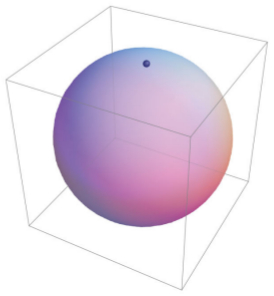
\includegraphics[scale=.3]{graphics/autonomy_static.jpg}
		\end{column}
		\begin{column}{0.3\textwidth}
			\centering
			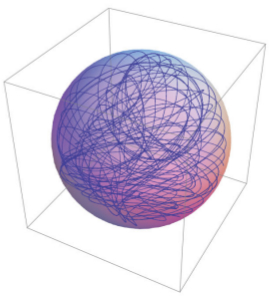
\includegraphics[scale=.3]{graphics/autonomy_chaotic.jpg}
		\end{column}
		\begin{column}{0.3\textwidth}
			\centering
			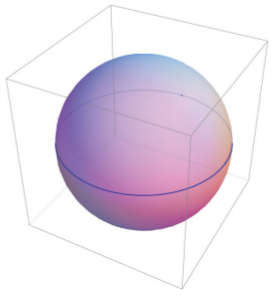
\includegraphics[scale=.3]{graphics/autonomy_simple.jpg}\,\cite{Tegmark_15_long}
		\end{column}
	\end{columns}
	\begin{itemize}
		\item{Reduktion der maximalen Energie-Kohärenz um wenige Prozent}
			\begin{itemize}
				\item{Komplexe, chaotische Dynamik möglich}
			\end{itemize}
	\end{itemize}}{}
\end{frame}
		
		
		
		
	
	\section{Zusammenfassung}
		\separatorslide
	\begin{frame}{Zusammenfassung}
	\large
	\begin{itemize}
		\item{Große Anzahl Regelungen und Gesetze}
		\begin{itemize}
			\item{strikte Meldepflicht}
		\end{itemize}
		\item{Sicherheitskonzepte}
		\begin{itemize}
			\item{Aufrechterhaltung der Barrieren}
			\item{Vielfache und vielseitige Ausführung von Sicherheitseinrichtungen}
			\item{passive Sicherheitseinrichtungen, wenn möglich}
		\end{itemize}
		\item{Vorbereitung für die Beherrschung eines Ernstfalls}
		\item{Regelmäßige Überprüfung, Instandhaltung und Verbesserung}
%		\item{Gefahr auch durch Kraftwerke im Ausland}
	\end{itemize}
\end{frame}
	
	
	\section*{Quellen}
	\separatorslide
	
	%\nocite{GRS,INES_Manual,bmud,BFS,kernenergieDE,wikiRS}
	\begin{frame}[allowframebreaks]{Quellen}
		\printbibliography
	\end{frame}

\end{document}